\documentclass[12pt]{article}


\usepackage{amsmath}
\usepackage[top=1in, bottom=1in, left=1.25in, right=1.25in]{geometry}
\usepackage{setspace}
\setcounter{secnumdepth}{1}
%\usepackage{tocstyle}
%\usetocstyle{standard}
\renewcommand{\contentsname}{\centerline {\normalsize Table of Contents}}
\usepackage{tocloft}
\renewcommand{\cftsecfont}{\normalsize}
\renewcommand{\cftsecleader}{\cftdotfill{\cftsecdotsep}}
\renewcommand\cftloftitlefont{\normalsize,\bfseries}
\renewcommand\cftlottitlefont{\normalsize,\bfseries}
\usepackage{sectsty}
\sectionfont{\normalsize}
\usepackage{enumitem}
\usepackage{natbib}
\usepackage{mathtools}
\usepackage{dsfont}
\usepackage{bm}
%\usepackage{cite}
\usepackage{float}
\usepackage{placeins}
\usepackage{adjustbox}
\usepackage{lscape}
\usepackage{caption}
%\usepackage{graphicx}	% Including figure files
\usepackage{amsmath}	% Advanced maths commands
\usepackage{amssymb}	% Extra maths symbols
\def\dd#1#2{\frac{d #1}{d #2}}
\def\2dd#1#2{\frac{d^2 #1}{d #2^2}}
\def\pd#1#2{\frac{\partial #1}{\partial #2}}
\def\2pd#1#2{\frac{\partial^2 #1}{\partial #2^2}}
\newcommand\sq{\mbox{\rlap{$\sqcap$}$\sqcup$}}% 
\newcommand\arcdeg{\mbox{$^\circ$}}% 
\newcommand\arcmin{\mbox{$^\prime$}}% 
\newcommand\arcsec{\mbox{$^{\prime\prime}$}}% 
\newcommand\fd{\mbox{$.\!\!^{\mathrm d}$}}% 
\newcommand\fh{\mbox{$.\!\!^{\mathrm h}$}}% 
\newcommand\fm{\mbox{$.\!\!^{\mathrm m}$}}% 
\newcommand\fs{\mbox{$.\!\!^{\mathrm s}$}}% 
\newcommand\diameter{\ooalign{\hfil/\hfil\crcr\mathhexbox20D}}% 
\newcommand\degr{\arcdeg}% 
\newcommand\Sun{\sun}% 
\newcommand\Sol{\sun}% 
\newcommand\sun{\odot}% 
\newcommand\Mercury{\astro{\char1}}% Mercury symbol, "1" 
\newcommand\Venus{\astro{\char2}}% Venus symbol, "2" 
\newcommand\Earth{\earth}% 
\newcommand\Terra{\earth}% 
\newcommand\earth{\oplus}% 
\newcommand\Mars{\astro{\char4}}% Mars symbol, "4" 
\newcommand\Jupiter{\astro{\char5}}% Jupiter symbol, "5" 
\newcommand\Saturn{\astro{\char6}}% Saturn symbol, "6" 
\newcommand\Uranus{\astro{\char7}}% Uranus symbol, "7" 
\newcommand\Neptune{\astro{\char8}}% Neptune symbol, "8" 
\newcommand\Pluto{\astro{\char9}}% Pluo symbol, "9" 
\newcommand\Moon{\astro{\char10}}% Moon symbol, "M" 
\newcommand\Luna{\Moon}% 
\newcommand\Aries{\astro{\char11}}% 
\newcommand\VEq{\Aries}% vernal equinox (Aries) 
\newcommand\Taurus{\astro{\char12}}% 
\newcommand\Gemini{\astro{\char13}}% 
\newcommand\Cancer{\astro{\char14}}% 
\newcommand\Leo{\astro{\char15}}% 
\newcommand\Virgo{\astro{\char16}}% 
\newcommand\Libra{\astro{\char17}}% 
\newcommand\AEq{\Libra}% autumnal equinox (Libra) 
\newcommand\Scorpius{\astro{\char18}}% 
\newcommand\Sagittarius{\astro{\char19}}% 
\newcommand\Capricornus{\astro{\char20}}% 
\newcommand\Aquarius{\astro{\char21}}% 
\newcommand\Pisces{\astro{\char22}}% 
\newcommand\ion[2]{#1$\;${%
\ifx\@currsize\normalsize\small \else
\ifx\@currsize\small\footnotesize \else
\ifx\@currsize\footnotesize\scriptsize \else
\ifx\@currsize\scriptsize\tiny \else
\ifx\@currsize\large\normalsize \else
\ifx\@currsize\Large\large
\fi\fi\fi\fi\fi\fi
\rmfamily\@Roman{#2}}\relax}% 

\newcommand\sbond{\chem@bnd{\@sbnd}}%
\newcommand\dbond{\chem@bnd{\@dbnd}}%
\newcommand\tbond{\chem@bnd{\@tbnd}}%

\graphicspath{{./}{Figures/}}

% Standard journal abbreviations
% Mostly as used by ADS, with a few additions for journals where MNRAS does not
% follow normal IAU style.

\newcommand\aap{A\&A}                % Astronomy and Astrophysics
\let\astap=\aap                          % alternative shortcut
\newcommand\aapr{A\&ARv}             % Astronomy and Astrophysics Review (the)
\newcommand\aaps{A\&AS}              % Astronomy and Astrophysics Supplement Series
\newcommand\actaa{Acta Astron.}      % Acta Astronomica
\newcommand\afz{Afz}                 % Astrofizika
\newcommand\aj{AJ}                   % Astronomical Journal (the)
\newcommand\ao{Appl. Opt.}           % Applied Optics
\let\applopt=\ao                         % alternative shortcut
\newcommand\aplett{Astrophys.~Lett.} % Astrophysics Letters
\newcommand\apj{ApJ}                 % Astrophysical Journal
\newcommand\apjl{ApJ}                % Astrophysical Journal, Letters
\let\apjlett=\apjl                       % alternative shortcut
\newcommand\apjs{ApJS}               % Astrophysical Journal, Supplement
\let\apjsupp=\apjs                       % alternative shortcut
% The following journal does not appear to exist! Disabled.
%\newcommand\apspr{Astrophys.~Space~Phys.~Res.} % Astrophysics Space Physics Research
\newcommand\apss{Ap\&SS}             % Astrophysics and Space Science
\newcommand\araa{ARA\&A}             % Annual Review of Astronomy and Astrophysics
\newcommand\arep{Astron. Rep.}       % Astronomy Reports
\newcommand\aspc{ASP Conf. Ser.}     % ASP Conference Series
\newcommand\azh{Azh}                 % Astronomicheskii Zhurnal
\newcommand\baas{BAAS}               % Bulletin of the American Astronomical Society
\newcommand\bac{Bull. Astron. Inst. Czechoslovakia} % Bulletin of the Astronomical Institutes of Czechoslovakia 
\newcommand\bain{Bull. Astron. Inst. Netherlands} % Bulletin Astronomical Institute of the Netherlands
\newcommand\caa{Chinese Astron. Astrophys.} % Chinese Astronomy and Astrophysics
\newcommand\cjaa{Chinese J.~Astron. Astrophys.} % Chinese Journal of Astronomy and Astrophysics
\newcommand\fcp{Fundamentals Cosmic Phys.}  % Fundamentals of Cosmic Physics
\newcommand\gca{Geochimica Cosmochimica Acta}   % Geochimica Cosmochimica Acta
\newcommand\grl{Geophys. Res. Lett.} % Geophysics Research Letters
\newcommand\iaucirc{IAU~Circ.}       % IAU Cirulars
\newcommand\icarus{Icarus}           % Icarus
\newcommand\japa{J.~Astrophys. Astron.} % Journal of Astrophysics and Astronomy
\newcommand\jcap{J.~Cosmology Astropart. Phys.} % Journal of Cosmology and Astroparticle Physics
\newcommand\jcp{J.~Chem.~Phys.}      % Journal of Chemical Physics
\newcommand\jgr{J.~Geophys.~Res.}    % Journal of Geophysics Research
\newcommand\jqsrt{J.~Quant. Spectrosc. Radiative Transfer} % Journal of Quantitiative Spectroscopy and Radiative Transfer
\newcommand\jrasc{J.~R.~Astron. Soc. Canada} % Journal of the RAS of Canada
\newcommand\memras{Mem.~RAS}         % Memoirs of the RAS
\newcommand\memsai{Mem. Soc. Astron. Italiana} % Memoire della Societa Astronomica Italiana
\newcommand\mnassa{MNASSA}           % Monthly Notes of the Astronomical Society of Southern Africa
\newcommand\mnras{MNRAS}             % Monthly Notices of the Royal Astronomical Society
\newcommand\na{New~Astron.}          % New Astronomy
\newcommand\nar{New~Astron.~Rev.}    % New Astronomy Review
\newcommand\nat{Nature}              % Nature
\newcommand\nphysa{Nuclear Phys.~A}  % Nuclear Physics A
\newcommand\pra{Phys. Rev.~A}        % Physical Review A: General Physics
\newcommand\prb{Phys. Rev.~B}        % Physical Review B: Solid State
\newcommand\prc{Phys. Rev.~C}        % Physical Review C
\newcommand\prd{Phys. Rev.~D}        % Physical Review D
\newcommand\pre{Phys. Rev.~E}        % Physical Review E
\newcommand\prl{Phys. Rev.~Lett.}    % Physical Review Letters
\newcommand\pasa{Publ. Astron. Soc. Australia}  % Publications of the Astronomical Society of Australia
\newcommand\pasp{PASP}               % Publications of the Astronomical Society of the Pacific
\newcommand\pasj{PASJ}               % Publications of the Astronomical Society of Japan
\newcommand\physrep{Phys.~Rep.}      % Physics Reports
\newcommand\physscr{Phys.~Scr.}      % Physica Scripta
\newcommand\planss{Planet. Space~Sci.} % Planetary Space Science
\newcommand\procspie{Proc.~SPIE}     % Proceedings of the Society of Photo-Optical Instrumentation Engineers
\newcommand\rmxaa{Rev. Mex. Astron. Astrofis.} % Revista Mexicana de Astronomia y Astrofisica
\newcommand\qjras{QJRAS}             % Quarterly Journal of the RAS
\newcommand\sci{Science}             % Science
\newcommand\skytel{Sky \& Telesc.}   % Sky and Telescope
\newcommand\solphys{Sol.~Phys.}      % Solar Physics
\newcommand\sovast{Soviet~Ast.}      % Soviet Astronomy (aka Astronomy Reports)
\newcommand\ssr{Space Sci. Rev.}     % Space Science Reviews
\newcommand\zap{Z.~Astrophys.}       % Zeitschrift fuer Astrophysik


\def\av#1{\left\langle #1 \right\rangle}
\def\braket#1#2{\left\langle#1|#1\right\rangle}
\def\opbraket#1#2#3{\left\langle #1\left|#2\right|#3\right\rangle}
\def\ket#1{\left|#1\right\rangle}
\def\cev#1{\reflectbox{\ensuremath{\vec{\reflectbox{\ensuremath{#1}}}}}}

\def\beq{\begin{equation}}
\def\eeq{\end{equation}}
\def\beqs#1\eeqs{\beq\begin{split} #1 \end{split}\eeq}

\usepackage{graphicx}
\graphicspath{{./}{Figures/}}

\usepackage{deluxetable}

%% Units
\def\fm {\,{\tt fm}}
\def\MeV {\,{\tt MeV}}
\def\GeV {\,{\tt GeV}}
\def\degC{\,{^\circ{\tt C}}}
\def\degK{\,{\tt K}}

\usepackage{microtype}
\usepackage[colorlinks=true,backref=false, linktocpage=true,
citecolor=blue,urlcolor=blue,linkcolor=blue,pdfpagemode=UseOutlines]{hyperref}

\hypersetup{%
  bookmarksnumbered=true,
  pdftitle = {},
  pdfsubject = {subject},
  pdfauthor = {Name of author},
  pdfkeywords = {keywords,separated, by, commas}
}


\begin{document}
\thispagestyle{empty}
\vspace*{1in}
\begin{center}
\center{Title of Dissertation\vspace*{36pt}}
\center{Name of Student\vspace*{36pt}}
\centerline{Previous Degree in Field, Month Year, School}
\centerline{Previous Degree in Field, Month Year, School}\vspace*{24pt}
\center{A Dissertation submitted to\vspace*{36pt}}
\begin{center}
The Faculty of\\The Columbian College of Arts and Sciences \\ of The George
Washington University\\ in partial fulfillment of the requirements\\ for the degree
of Doctor of Philosophy\\[36pt]
Month Day, Year\\[36pt] %date of degree conferral 
Dissertation directed by\\[\baselineskip]
Name of Director\\
Position\\[\baselineskip]
Name of Co-director\\
Position
\end{center}
\end{center}
% display page numbers in the footer and centered. Start with roman numerals %
\pagestyle{plain}
\setcounter{page}{1}
\pagenumbering{roman}
\newpage
\begin{doublespace}
\noindent
The Columbian College of Arts and Sciences of The George Washington University certifies that \texttt{Name of Student} has passed the Final Examination for the degree of Doctor of Philosophy as of \texttt{date of defense}. This is the final and approved form of the dissertation.
\end{doublespace}
\vspace{12pt}
\begin{center}
Title of Dissertation

\vspace*{36pt}
Name of Student
\vspace{24pt}
\end{center}
Dissertation Research Committee:
\vspace{12pt}

\indent Name of Director, Position, Dissertation Director
\vspace{12pt}

\indent Name of Co-director, Position, Dissertation Co-Director
\vspace{12pt}

\indent Name of Reader, Position, Committee Member
\vspace{12pt}

\indent Name of Reader, Position, Committee Member
\vspace{12pt}
%only readers and directors are listed per CCAS. No examiners or chairs.

\newpage
\phantomsection \label{dedication}
\begin{center}
\section*{\textbf{Dedication}}
\end{center}
\addcontentsline{toc}{section}{\textbf{Dedication}}
\begin{center}
\vspace*{6pt}
%\vspace*{-24pt}
Dedication text goes here.

\end{center}

\doublespacing
\newpage
\phantomsection \label{acknowledgements}
\begin{center}
\section*{Acknowledgments}
\end{center}
\vspace*{6pt}
\addcontentsline{toc}{section}{\textbf{Acknowledgements}}
So long, and thanks for all the fishes.
\doublespacing
\newpage
\begin{center}
\section*{Abstract of Dissertation}
\end{center}
\phantomsection \label{abstract}
\addcontentsline{toc}{section}{\textbf{Abstract of Dissertation}}
\vspace*{-40pt}
\vspace{24pt}
\begin{singlespace}
\center{Title of Dissertation}
\end{singlespace}
\vspace{-12pt}
\vspace*{24pt}
Abstract goes here.
\doublespacing
\newpage
\tableofcontents
\newpage
\cleardoublepage
%\fi

%\iffalse
\phantomsection \label{listoffig}
\addcontentsline{toc}{section}{\textbf{List of Figures}}
\begin{center}
\listoffigures
\end{center}
\newpage
%\fi

%\iffalse
\cleardoublepage
\phantomsection \label{listoftab}
\addcontentsline{toc}{section}{\textbf{List of Tables}}
\begin{center}
\listoftables
\end{center}
\newpage
%\fi

\begin{center}
\section*{\textbf{List of Symbols}}
\end{center}
\addcontentsline{toc}{section}{\textbf{List of Symbols}}

\subsection*{General Units}
\begin{itemize}
    \item[]pc Parsec ($3.26$ly)
    \item[]ly Lightyear ($9.461\times 10^{17}$cm)
    \item[]$c$ Speed of Light
    \item[]$M_{\odot}$ Solar Mass ($1.99\times10^{33}$g)
    \item[]$R_{\odot}$ Solar Radius ($6.96\times10^{10}$cm)
    \item[]$L_{\odot}$ Solar Luminosity ($3.826\times10^{33}$erg/s)
    \item[]foe $10^{51}$erg
\end{itemize}

\newpage

\iffalse
\section {\protect \centering Glossary of Terms(optional)}
\doublespacing
\begin{itemize}
\addtolength{\itemindent}{0.25in}
\item[Term 1]: Start Definiton here
\item[Term 2]: Start Definiton here
\end{itemize}
\newpage
\pagenumbering{arabic}
\fi



 
   
         
       
%----------------------------------------------------------------------------------------
%	ARTICLE CONTENTS
%----------------------------------------------------------------------------------------
 \doublespacing
\setcounter{page}{1}
%\vspace*{-2cm}
\pagenumbering{arabic}
\section{Introduction}
\label{introlabel}
The wonderful introduction you will write.
\newpage
\section{Science}
\label{chapterlabel}
All the amazing science you did goes here.

\subsection{Subsection of Science}
Details of your amazing work. This is a reference to Table \ref{tab:snlx}
\subsubsection{More Details}
\paragraph*{}
\singlespacing
\begin{deluxetable}{lccccr}
\tablecolumns{9}
\tablewidth{0pc}
\tablecaption{Example of a Deluxe Table \label{tab:snlx}}
\tablehead{
\colhead{SNe} & \colhead{Obs ID} & \colhead{Distance} & \colhead{t$_{\mathrm{obs}}$\tablenotemark{a}} & \colhead{L$_{\mathrm{X}}$\tablenotemark{b}}  & \colhead{Reference} \\
\colhead{} & \colhead{} & \colhead{Mpc} & \colhead{yr} & \colhead{10$^{38}$ ergs s$^{-1}$}  & \colhead{}
}
\startdata
SN 1957D & & 4.61 & 43 & $\leq 10.65$& \citep{long12}\\ 
 & & & 49 & $\leq 6.83$ & \\ 
 & & & 55 & $6.15^{+5.06}_{-1.08}$& \\ 
SN 1970G & & $7.4^{+1.0}_{-1.5}$ & 20.9 & 4.9$\pm$ 1.1& \citep{Dittman14}\\ 
 & & & 26.1 & 2.6$\pm$ 0.6& \\ 
 & & & 34.0 & 1.1$\pm$0.2& \\ 
 & & & 41.6 & 4.1$\pm$ 1.2& \\ 
SN 1979C\tablenotemark{*} & & 15.34 & 0.7 & 6.3$\pm$ 1& \citep{Patnaude11}\\ 
 & & & 16.2 & 8.2$\pm$ 0.9& \\ 
 & & & 20.6 & 6.9$\pm$ 0.6& \\ 
 & & & 22.7 & 6.3$\pm$ 0.7& \\ 
 & & & 26.5 & 6.3$\pm$ 0.7& \\ 
 & & & 26.9 & 6.6$\pm$ 0.5& \\ 
 & & & 28.0 & 7.0$\pm$ 0.5& \\ 
 & & & 31.0 & 5.7$\pm$ 0.5& \\ 
 & & & 32.0 & 6.3$\pm$ 0.4&  
\enddata
\tablenotetext{a}{Observations are taken as time since CC (generally time since first observation).}
\tablenotetext{b}{X-ray luminosity is for the 0.1 -- 10 keV range.}
\tablenotetext{*}{X-ray luminosity is for the 0.3 -- 2.0 keV range.}
\end{deluxetable}
\newpage
\section{Conclusions}
\label{conc}
\subsection{Summary}
This is what I did...
\subsection{Future Work}
This would be good to do...

\newpage
\section{References}
{\def\section*#1{}
\singlespacing
\bibliographystyle{aasjournal}
\bibliography{bibliography}
}
\newpage
\newgeometry{top=1in, bottom=1in, left=1.25in, right=1.25in}



\doublespacing
\appendix


\section{Appendix}\label{appendixlabel}
Figure \ref{fig:snr_pipeline} is an example figure.
\begin{figure}[htb!]
    \centering
    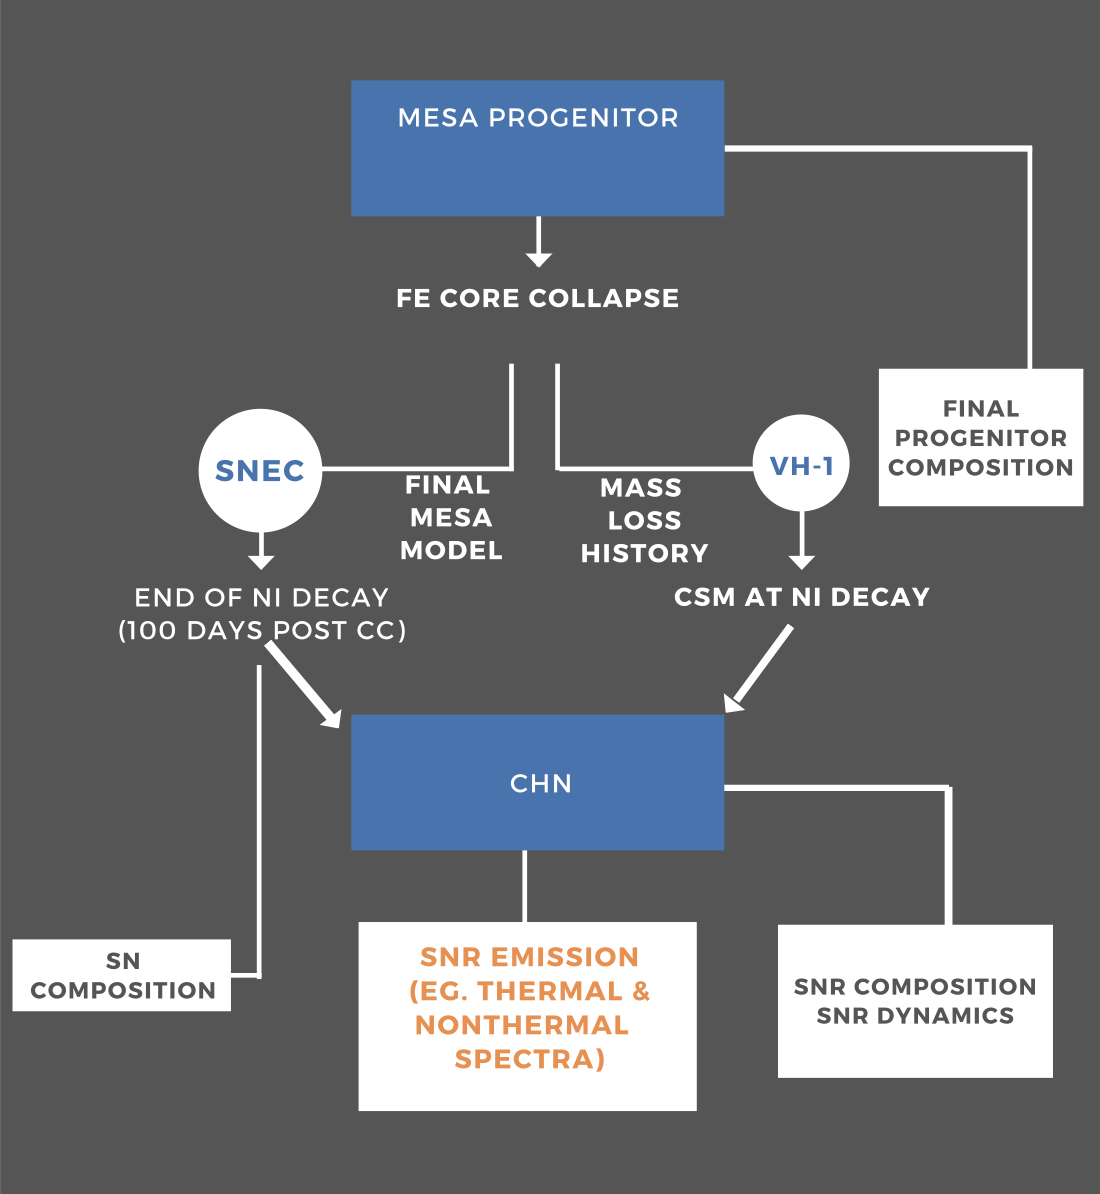
\includegraphics[width=\textwidth]{SNR_pipeline.png}
    \caption{Example figure}
    \label{fig:snr_pipeline}
\end{figure}


\end{document}

